\section{Preliminaries} \label{sec:Preliminaries}
This section gives a short introduction to cryptographic constructs necessary for a thorough understanding of the protocol. In particular, the proof-of-work scheme and Merkle trees will be discussed. Note that Digital Signatures are required as well but are intentionally skipped for they are sufficiently covered by online literature.

\subsection{Proof of Work} \label{sec:ProofOfWork}
A proof-of-work is a cryptographic puzzle used to ensure that a party has performed a certain amount of work. In particular, the Bitcoin mining process (see Sect. \ref{sec:Mining}) incorporates a proof-of-work system based on Adam Back's Hashcash \cite{Back_Hashcash}. It has two basic properties - firstly, it ensures that the party providing the proof-of-work has invested a predefined amount of effort in order to create the proof and secondly, that the proof is efficiently verifiable. Typically, finding a solution proof-of-work puzzle is a probabilistic process with a success probability depending on the predefined difficulty.

Let Alice and Bob be two parties communicating with each other and let Alice require Bob to perform a certain amount of computational work for each message he sends to Alice. To do so, Alice can require Bob to provide a string whose one-way hash satisfies a predefined structure. Finding such a string has a certain success probability that will determine how much work Bob has to invest on average in order to find a valid solution.

For example, in Bitcoin the hashing algorithm is \emph{double-SHA256} ($\mathit{SHA256^{2}}$) and the predefined structure is a hash less or equal to a target value \emph{T}. The success probability of finding a nonce \emph{n} for a given message \emph{msg}, such that $\mathit{H = SHA256^{2}(msg||n)}$ is less or equal to the target \emph{T} is
\begin{equation}
Pr[H \leq T] = \frac{T}{2^{256}}.
\end{equation}

\newpage
\noindent
This will require a party attempting to find a proof-of work to perform, on average, the following amount of computations
\begin{equation}
\frac{1}{Pr[H \leq T]} = \frac{2^{256}}{T}.
\end{equation}

\noindent
Finally, it is easy to see that it can be efficiently verified whether the nonce accompanied with the message is indeed a valid proof-of-work by simply evaluating
\begin{equation}
SHA256^{2}(msg||n) \leq T.
\end{equation}


\subsection{Merkle Trees} \label{sec:MerkleTrees}
Merkle trees, named after their creator Ralph Merkle, are binary hash trees used for efficient verification of data integrity. An example of a Merkle tree can be seen in Fig. \ref{fig:MerkleTree}. Leaves are computed directly as hashes over data blocks, whereas nodes further up the tree are computed by concatenating and hashing their respective children.

\begin{figure}[htbp]
 \centering
 \includegraphics[scale=0.75]{images/MerkleTree.pdf}
 \caption{Merkle Tree}
 \label{fig:MerkleTree}
\end{figure}
\vspace{-10pt}

\noindent
The main advantage of Merkle trees is that when one data block changes it is not necessary to compute a hash over all the data, as opposed to naive hashing. Assume data block $\mathit{d_{00}}$ is modified, then $\mathit{n_{00}}$ has to be re-computed as well as all nodes along the branch until the root node. Therefore, the number of required hash computations scales logarithmically in the number of data blocks. Since both data blocks and hashes are relatively small in size, this process is fairly efficient.

\subsubsection*{Other cases}
The previously discussed example considered the situation where the number of data blocks is a power of two. In such a case the computation results in a full and complete binary tree. However, since it is required that each node, except for the leaves, has exactly two children, measures have to be taken if nodes are missing. In the following the method used in Bitcoin will be discussed.

\noindent
The solution is straightforward - when forming a row in the tree (excluding the root), whenever there is an odd number of nodes, the last node is duplicated. In effect, each intermediary row in the tree will always have an even number of nodes and therefore each node, except for the leaves, will have exactly two children.

\begin{figure}[htbp]
 \centering
 \includegraphics[scale=0.75]{images/MerkleTree2.pdf}
 \caption{Merkle Tree with Missing Nodes}
 \label{fig:MerkleTree2}
\end{figure}
\vspace{-10pt}

\noindent
In the example given in Fig. \ref{fig:MerkleTree2} there are only three data blocks and therefore the computation of the fourth node in the second row is missing a child. Thus, the last node is replicated and the computation is continued as in the previous example (see Fig. \ref{fig:MerkleTree}). Should an odd number of nodes occur at any other point during the computation, then the same rule is applied.